\subsection{Display Module (DP) }
\label{sec:DP}
The Display Module (DP) presents information on the ongoing metering process. This includes:

\begin{itemize}
    \item timestamp: current date and time
    \item process state: accumulating, transmitting, requesting internet time, ...
    \item power: battery voltage, solar panel voltage
    \item SD-Card reader: current filename
\end{itemize}

\subsubsection{Requirements}
We noticed the importance of providing comprehensive diagnostic information at the location of deployment.
The hardware is located inside a street gully which is exposed to humidity, dirt and mosquitos. When inspecting the system, the technician
must be able to diagnose a potential problem at a glance. He must be able to quickly decide if the unit must be dismounted and sent to the lab.
The display must therefore be clearly visible from every angle. This excludes LCD displays.
Given the absence of grid-connection, low power consumption is mandatory. This excludes LED displays.

\subsubsection{Implementation}
We use a small,
inexpensive OLED with very low power consumption of only \qty{30}{\nA}.
\begin{figure}[h]
    \centering
    \includegraphics[width=0.2\textwidth]{MA/DP/DP}

\end{figure}


\begin{table}[H]
    \centering
    \begin{threeparttable}[b]
        \begin{tabularx}{\linewidth}{ >
                    {\hsize=.25\hsize}X >
                    {\hsize=0.5\hsize}X >
                    {\hsize=.25\hsize}X  >
                    {\hsize=.5\hsize}X >
                    {\hsize=.25\hsize}X  >
                    {\hsize=3\hsize}X
            }
                  & \multicolumn{4}{c}{Pin mapping} &                                                    \\
            \cmidrule(lr){3-6}
            Id    & Net                             & Nb. & Name         & Type               & Function \\
            \midrule
            $U_1$ & .3V3                            & 4   & \texttt{VCC} & \rightharpoonup    &          \\
            $U_1$ & .GND                            & 5   & \texttt{GND} & \rightharpoonup    &          \\
            $U_1$ & .SCL                            & 6   & \texttt{SCL} & \leftharpoonup     &          \\
            $U_1$ & .SDA                            & 7   & \texttt{SDA} & \leftrightharpoons &          \\
        \end{tabularx}
    \end{threeparttable}
\end{table}


\begin{table}[H]
    \centering
    \begin{tabularx}{\linewidth}{>{\hsize=0.25\hsize}X
            >{\hsize=1\hsize}X >{\hsize=1\hsize}X
            >{\hsize=0.5\hsize}X >{\hsize=2.25\hsize}X}
        Id    & BOM Item                 & Order Code  & Package & Rationale     \\
        \midrule
        $U_1$ & \cite{noauthor_096_2021} & WPI438 / 59 & DIL (4) & I2C interface \\
    \end{tabularx}


\end{table}